\chapter{Preface}

I first became interested in vehicle dynamics through involvement with my college Formula SAE team.  I was on summer break after finishing my freshman year, and somehow I stumbled upon the team's website.  Racecars!  Cool!  So the next weekend, after some e-mails back and forth, I set out to a local autocross where the team was cooking burgers and hot dogs as a fundraiser.  Cars of all kinds racing through a sea of orange cones.  Having never been to an autocross before, I was curious.  ``Why is it that some cars lift the front wheel in the corners, and others lift the rear wheels?''  ``How come the real racecars don't screech tires like the street cars do?''

It didn't take long before it was clear that I had caught the racecar bug.  I was particularly drawn to suspensions.  I'm not entirely sure why that was, maybe because you could see all of the moving parts, or maybe because there was an experienced alumni who spent a lot of time in the shop who was also interested in suspension design.  Anyway, we spent many hours discussing vehicle dynamics and suspension design, pouring through the team's library of reference material and studying suspension kinematics with the help of purpose-built commercially available software.

The software we were using had terrible graphics and was somewhat tedious to use, but it provided accurate results and was simple enough to be confident that we provided the correct input.  It only permitted kinematic analysis of the suspension, and only one end of the car at a time, but it seemed well suited to our needs.  As I gained more experience and started to search for justification of more design decisions, it became clear that this software had some shortcomings.  At the time, it was our only option and many of the other engineering packages we used also had shortcomings.  Most of the time, it was easy to accept the issues and work around them.

In the summer of 2005, immediately following the conclusion of the 2005 FSAE season, a good friend of mine, Matt Jarvis, began work on redesigning the frame to be stiffer and lighter.  Matt was (and still is) a brilliant engineer.  Among his interests were programming, finite element analysis and composites.  He had taken the lead on the bodywork the previous year and wanted to consider adding composite panels to the frame design.  We had previously used aluminum panels for this purpose, bonding and riveting them to the frame.  Matt knew that a composite solution could improve the design, but it introduced several variables that we hadn't had to consider before.

Traditionally, someone would create a finite element model of the frame and apply a virtual torsional load.  The displacement was calculated by the finite element software from which a stiffness could be calculated.  The stiffness was compared to the weight to determine the overall quality of the design.  Then the designer would look at the stresses in the frame members and adjust the geometry and/or the cross section of certain members, with the goal of improving stiffness and reducing weight.  This process would continue until the designer stopped making progress or ran out of time.  Then they'd just pick the frame that had the best stiffness to weight ratio, and start fabrication.

Matt looked at this problem and saw all of the available permutations.  Even if you assumed the geometry was fixed, the number of frame members multiplied with the number of available cross sections (round, square, rectangular, dimensions, wall thickness) meant there was an incredible number of possible combinations.  He wrote VBA macros into excel spreadsheets that implemented a genetic search algorithm to intelligently evaluate a huge number of these permutations and hopefully converge on a solution.  After commandeering the computer lab overnight to run the optimization in parallel on some 20 machines, nearly 100,000 frame designs had been simulated.  The best design was both stiffer and lighter than the best human-designed frame from the previous year.  I was incredibly impressed by his success.

Also for the 2005-06 FSAE season, we decided to set the springs and dampers side-by-side instead of using coil-overs in an attempt to reduce the bending load on the damper shafts.  In theory, this would reduce friction in the damper and give us more control over the damping characteristics of the suspension.  This meant spending twice as much effort at each end to ensure the bellcrank geometry gave us the desired installation ratios across the entire range of motion.  Unfortunately, this was also one of the more tedious jobs to tackle with our suspension kinematics software.  Ideally, the designer would be able to look at the bellcrank along it's pivot axis, giving a clear view of the angles between the pushrod, bellcrank and spring or damper, and how they change through the range of motion.  Or better yet - show a plot of the installation ratio across the desired range of motion, updated dynamically as the bellcrank design was adjusted.  Also, it is important that all of these points lie on a common plane.  Our suspension package did not permit either of the above.  Our work-around was to bounce back-and-forth between our CAD software and the suspension design software.  This was not going to be a fun task.

After spending several hours trying to work out the bellcrank geometry, I thought I would try to solve the kinematics problem myself, creating a tool that was designed exactly for the problem at hand.  A few hours later, I had written some VBA code in an Excel spreadsheet that elegantly solved the problem of designing bellcrank geometry.  Even with the time invested in the creation of the tool, the total time to design new bellcranks had been reduced and the results were probably better than what would have been achieved with our prior workflow.  I experienced a great feeling of satisfaction, attached more to the creation of a useful tool than completing the design of the bellcranks.

Following my success with my bellcrank spreadsheet, I became interested in attempting to simulate the dynamics of the entire racecar.  With good tire data and mass properties data, we could simulate the car performing maneuvers and quantify how changes in \emph{anything} would affect lap times.  In December 2005 I took a stab at writing software that would model a full vehicle - tires, suspension, engine, brakes, etc.  I was extremely naive and this effort stopped only weeks after it started.  It would have been a much better use of my time to focus on the manufacturing of our racecar (apologies to my 2005-06 team members!).

\begin{figure}
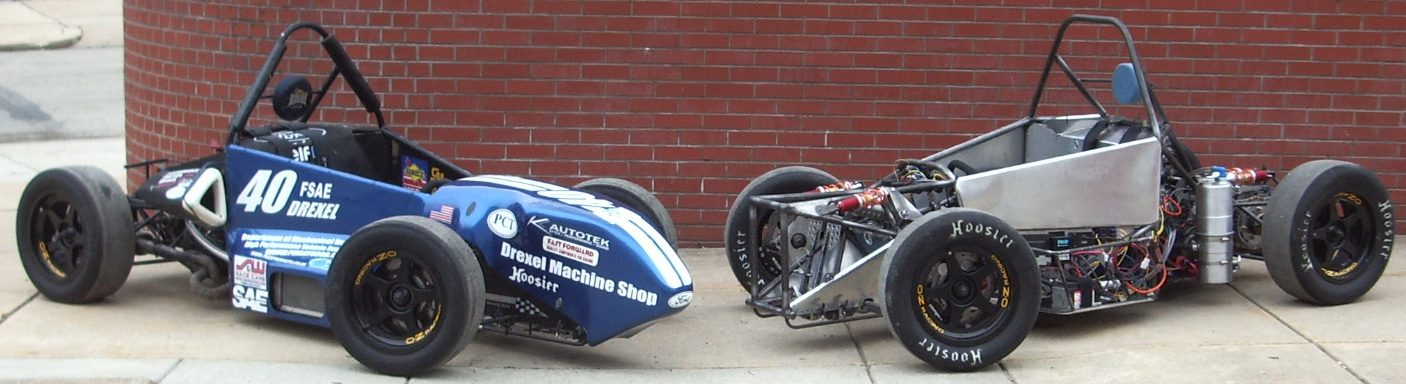
\includegraphics[width=\textwidth]{images/04-05cars}
\caption{The 2004 and (incomplete) 2005 Drexel University entries into the Formula SAE competitions}
\centering
\end{figure}

After graduating in 2007, I began work on what became the first incarnation of \vvase{}.  It was a simple application that could solve the vehicle kinematics problem for double A-arm suspensions.  I had made some improvements over the bellcrank spreadsheet I created a couple years earlier - it was faster, more accurate and more robust.  But it didn't do anything more than what other commercially available suspension kinematics software could do - in fact, in most ways it did less.  It was a learning exercise for me, but it wasn't very valuable as a tool.

At some point, I thought back to the genetic search algorithm that Matt had used to optimize the frame design.  Could something similar be applied to suspension kinematics?  After some careful thought and many hours of programming, I finally had something that was unique.  As far as I knew, there was no commercially available suspension kinematics package that could do an optimization like \vvase{}.

Although I never pursued a job in the auto industry, my FSAE experience became a significant influence on my career.  In addition to my engineering tasks associated with delivering our products, I develop special-purpose software tools for solving problems unique to our products and workflows.  I still have an interest in vehicle dynamics and racing, but I was surprised to find that I have a passion for creating tools.  This passion is what has driven me to continue work on \vvase{}, years after it began as an exercise and an experiment.  I hope that it satisfies other's needs to analyze suspension kinematics in the same manner it has satisfied my desire to create a tool.

% Influence of this experience on work (CAD tools, simulation, etc.)
% Influence of work experience back on this

%engineering problems are broad
%software is powerful and flexible, but requires expertise in both field and s/w usage.  confidence in inputs, confidence in output interpretation

%better decisions faster

\needspace{4\baselineskip}
\begin{flushright}
Kerry R. Loux \\
Langhorne, PA \\
July 2015
\end{flushright}
